The Barnes-Hut algorithm works by using an adaptive quadtree, which is shown in Figure~\ref{fig:sep}. In this figure, each color represents one ``branch'' of the quadtree. The blue branch is refined more than the others due to the point located in it. It is known as an {\em adaptive quadtree} because it only refines the grid up to the point where particles can be approximated reasonably well as a single particle.

\begin{figure}[H]
\centering
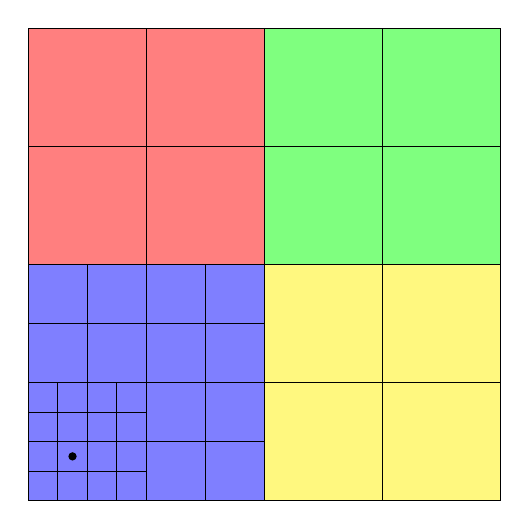
\begin{tikzpicture}[scale=.75]
\draw (0,0) -- (8,0) -- (8,8) -- (0,8) -- (0,0);
\filldraw[fill=green, draw=black, fill opacity=0.5] (4,4) rectangle (8,8);
\filldraw[fill=red, draw=black, fill opacity=0.5] (0,4) rectangle (4,8);
\filldraw[fill=yellow, draw=black, fill opacity=0.5] (4,0) rectangle (8,4);
\filldraw[fill=blue, draw=black, fill opacity=0.5] (0,0) rectangle (4,4);
\draw (2,0) -- (2,8);
\draw (6,0) -- (6,8);
\draw (0,2) -- (8,2);
\draw (0,6) -- (8,6);
\draw (1,0) -- (1,4);
\draw (3,0) -- (3,4);
\draw (0,1) -- (4,1);
\draw (0,3) -- (4,3);
\draw (.5,0) -- (.5,2);
\draw (1.5,0) -- (1.5,2);
\draw (0,.5) -- (2,.5);
\draw (0,1.5) -- (2,1.5);
\fill (.75,.75) circle (2pt);
\end{tikzpicture}
\caption{Adaptive Quadtree}
\label{fig:sep}
\end{figure}

To approximate the single particle, the center of mass is calculated for all the particles in that octant. The total mass in that octant would be the sum of the masses. In other words:

\begin{align}
\vec{r}_{i} = \frac{\sum_{i=1}^{\zeta}m_{i}\vec{x}_{i}}{\sum_{i=1}^{\zeta}m_{i}}
\end{align}

where $\zeta$ is the total number of particles in the given octant. This new position and mass are used to approximate the particles that are reasonably far enough away to be approximated as a single point.

The colors in Figure~\ref{fig:quadtree} represent those particles that are ``far enough away.'' Those in red are approximated as larger particles, and they decrease in size as you go down to finer grains. The larger the particles in the grid, the more that were approximated/averaged in that octant. The ones in the yellow grid are down to the finest grain size where each dot represents a single particle. The finest octant size is given for those in yellow, which are the octant's neighbors. 

\begin{figure}[H]
\centering
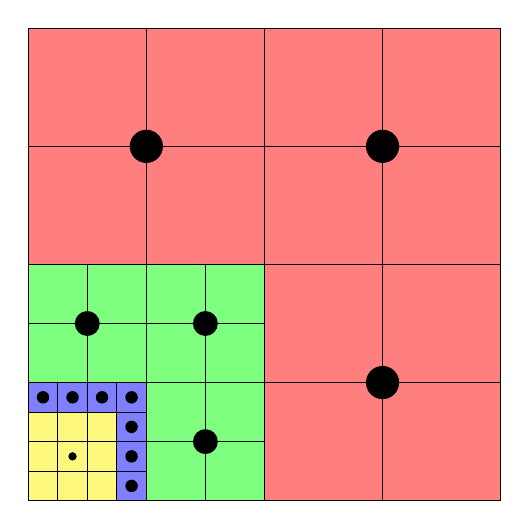
\begin{tikzpicture}[scale=.75]
\draw (0,0) -- (8,0) -- (8,8) -- (0,8) -- (0,0);
\filldraw[fill=red, draw=black, fill opacity = .5] (0,0) rectangle (8,8);
\filldraw[fill=white, draw=black] (0,0) rectangle (4,4);
\filldraw[fill=green, draw=black, fill opacity = .5] (0,0) rectangle (4,4);
\filldraw[fill=white, draw=black] (0,0) rectangle (2,2);
\filldraw[fill=blue, draw=black, fill opacity = .5] (0,0) rectangle (2,2);
\filldraw[fill=white, draw=black] (0,0) rectangle (1.5,1.5);
\filldraw[fill=yellow, draw=black, fill opacity = .5] (0,0) rectangle (1.5,1.5);
\draw (4,0) -- (4,8);
\draw (0,4) -- (8,4);
\draw (2,0) -- (2,8);
\draw (6,0) -- (6,8);
\draw (0,2) -- (8,2);
\draw (0,6) -- (8,6);
\draw (1,0) -- (1,4);
\draw (3,0) -- (3,4);
\draw (0,1) -- (4,1);
\draw (0,3) -- (4,3);
\draw (.5,0) -- (.5,2);
\draw (1.5,0) -- (1.5,2);
\draw (0,.5) -- (2,.5);
\draw (0,1.5) -- (2,1.5);
\fill (.75,.75) circle (2pt);
\fill (2,6) circle (8pt);
\fill (6,6) circle (8pt);
\fill (6,2) circle (8pt);
\fill (1,3) circle (6pt);
\fill (3,3) circle (6pt);
\fill (3,1) circle (6pt);
\fill (1.25,1.75) circle (3pt);
\fill (.75,1.75) circle (3pt);
\fill (.25,1.75) circle (3pt);
\fill (1.75,1.75) circle (3pt);
\fill (1.75,1.25) circle (3pt);
\fill (1.75,.75) circle (3pt);
\fill (1.75,.25) circle (3pt);
\end{tikzpicture}
\caption{Adaptive Quadtree Coarsening}
\label{fig:quadtree}
\end{figure}

The code can be found \cite{github} under the github branch {\tt CS6320\_Semester\_Project}. The complexity of building the tree in {\sc Dendro} is $\mathcal{O}\left( \frac{N}{p}\log\left( N/p\right)\right)$. Since the positions of the particles are updated after each time step, the octants change as well. This can be prevented by altering/adjusting the tree after each time step. However, the implementation that was used was rebuilding the tree after each iteration. Therefore, the {\em time complexity} is $\mathcal{O}\left( t \frac{N}{p}\log\left( N/p\right)\right)$, where $t$ is the number of time steps.

{\sc Dendro} is ``probably, yea'' work-optimal \cite{milinda}. The calculation part is work optimal as it can be parallelized easily and not have to do any extra work.
